\documentclass[a4paper, 11pt]{article}
\usepackage[utf8]{inputenc}
\usepackage{subcaption}
\usepackage{parskip}
\usepackage[T1]{fontenc}
\usepackage{lmodern}
\usepackage[square,numbers]{natbib}
\usepackage{graphicx, float}
\usepackage{etoolbox}
\usepackage{url}
\usepackage{mathtools}
\usepackage[capitalize]{cleveref}
\usepackage[inkscapelatex=false]{svg}
\floatstyle{ruled}
\newfloat{program}{thp}{lop}
\floatname{program}{Program}

\graphicspath{{assets/}}

% red outline box
\renewcommand\fbox{\fcolorbox{red}{white}}

\renewcommand{\thesection}{\arabic{section}}
\renewcommand{\thesubsection}{\thesection.\arabic{subsection}}
\renewcommand{\thesubsubsection}{\thesubsection.\arabic{subsubsection}}

\makeatletter
\renewcommand{\@seccntformat}[1]{{\csname the#1\endcsname}.\enspace}
\patchcmd{\section}{\scshape}{\bfseries}{}{}
\patchcmd{\subsection}{\itshape}{\bfseries}{}{}
\patchcmd{\subsubsection}{\itshape}{\bfseries}{}{}
\makeatother

\newcommand{\wideimage}[2][]{%
  \makebox[\textwidth][c]{\includegraphics[width=1.2\textwidth,#1]{#2}}%
}

% eg etc ie implementation
\makeatletter
\newcommand{\ie}{\emph{i.e.}\@ifnextchar.{\!\@gobble}{}}
\newcommand{\eg}{\emph{e.g.}\@ifnextchar.{\!\@gobble}{}}
\newcommand{\etc}{etc\@ifnextchar.{}{.\@}}
\makeatother

\newcommand{\mica}{\textit{MICA }}

\title{MICA: Missing Imputation Comparison Analysis}
\author{Tharun Tilakumara \\ 220424448}
\date{\today}

\begin{document}

\begin{titlepage}
    \centering
    \vspace*{1cm}
    
\includegraphics[width=0.6\textwidth]{uniLogo.png}\\[2cm]
    
    {\Huge \bfseries MICA: Missing Imputation Comparison Analysis\par}
    \vspace{1cm}
    {\LARGE B.Sc. Computer Science\par}
    \vspace{2cm}
    
    {\Large \textbf{Tharun Tilakumara}} \\[0.5cm]
    {\Large 220424448} \\[2cm]
    
    {\large Supervised by: Sara Johansson Fernstad} \\
    {\large Word Count: 0xDEADBEEF}
    
    {\Large \today}
\end{titlepage}

\onecolumn 

\section*{Abstract}
This is an example of how to cite references \cite{little_statistical_2019}.
To-do
Another citation afoot! \cite{little_statistical_2019}
\newpage


\pagenumbering{arabic}
\tableofcontents
\newpage

\section{Introduction}
\subsection{Motivation}
The workflow of a data-scientist typically follows the following order of
tasks. 
\begin{enumerate}
        \item Capturing of data
        \item Preprocessing of data 
        \item Exploratory analysis 
        \item Final analysis 
\end{enumerate}

The majority of time out of this workflow is consumed by the preprocessing of
data step. As shown in \cite[p~3 fig~2]{sarih_data_2019} the cleaning and
organizing of data takes up an estimated 60\% of a data-scientists time. This
is a manual process that requires human judgement. This critical step requires
tedious and rigorous testing; In particular, low-quality data imputation can
result in unnatural or even worse, misleading distributions of values. The side
effects of which can include poorly performing prediction models and inaccurate
exploratory and final analysis. Data imputation started with simple methods
such as mean/median imputation. With the discovery of the mechanics of missing
data and concepts such as MCAR (missing completely at random), MAR (missing at
random) and MNAR (missing not at random) \cite{little_statistical_2019}, data
scientists now have access to a large array of complex algorithms to choose
from, which each have their own positives and drawbacks. Picking the optimal
algorithm for imputation for each feature in a dataset is time-consuming and
prone to error. 

While applications in the past have been developed to ease data imputation,
such as VIM \cite{templ_exploring_2012}, MANET \cite{unwin_interactive_1996}
and AmeliaView \cite{honaker_amelia_2024}, there has been little development in
the way of comparing different imputations of the same dataset. Currently, the
solution for comparing different imputation results would be to manually create
separate scripts for each imputation method and then, using the created
versions of the datasets, compare them using graphs. 

Older applications, such as the ones
mentioned before lack newly discovered visualization methods such as MissiG
\cite{fernstad_explore_2022} that could prove to be more useful for analyzing
missingness of data. 

\subsection{Aims} 

This project aims to:
\begin{itemize} 

        \item Make the decision-making step for data imputation easier by
                providing a touch screen dashboard interface for comparing
                different imputation results that are derived from different
                algorithms of imputation. 

        \item Reduce the time spent on the preprocessing of datasets as well as
                improve the results of imputed datasets.

        \item Create a solution for keeping track of combinations of
                imputations performed on versions of datasets created from
                prior imputations in a GIT \cite{noauthor_git_nodate} style
                version control system. 

\end{itemize}

\subsection{Objectives}

\begin{enumerate}

\item \textbf{Missingness Structures} - This dissertation will investigate and
        explain the concept of missingness structures and its role in data
        imputation and analysis. It will explain the different types of missing
        data as well as provide examples via synthetically created missing
        data.

\item \textbf{Missing Data Visualizations} - This dissertation will talk about
        methods of missing data visualizations. It will also provide
        implementations of discussed visualizations. 
        
\item \textbf{Imputation Version Control} - This dissertation will propose a
        method of keeping track of imputed datasets, discussing an example
        use case as well as implementation details.

\item \textbf{Web App Implementation and User-flow} - The main created artifact
        of this dissertation is a web app to impute and compare imputed
        datasets. Features and an example user-flow will be presented.

\end{enumerate}

\subsection{Dissertation Structure}
To-do

\newpage

\section{Background Review}
This part covers the background research gone into the design of the main
artifact \emph{MICA} and the synthetic missing data generator.
\subsection{The Nature of Missing Data Structures}

For the below figure examples, the UCI Irvine Heart Disease dataset
\cite{andras_janosi_heart_1989} was used as a base with missingness mechanisms
and patterns synthetically added after. 

There are two parts to go over for understanding how to tackle missing data. 
\begin{enumerate}
        \item \textit{Missingness mechanisms}
        \item \textit{Missingness patterns}
\end{enumerate}

\subsubsection{Missingness mechanism}
As explained in \cite{rubin_inference_1976}, a missingness mechanism is defined
as why data is missing depending on other variables observed as well as the
missing variable itself. Analyzing why data is missing is crucial in finding
the best method of to deal with missing values as if we were to assume data is
always \textit{Missing Completely at Random}, we can skew distributions of
features unintentionally. We have three categories to describe the types of
missingness mechanisms.

\paragraph{\textbf{Missing Completely at Random (MCAR)}}~\\ 
MCAR is a missingness mechanism where missing values are not related to other
recorded or unrecorded data. This is the least severe of the three missingness
mechanisms as you are able to impute the dataset without causing large
unintended side effects without knowing the underlying mechanism of why the
data is missing. Dropping records with missing values will not affect the
distribution of the variables greatly. \eg
\cref{fig:distribution_lines_age_MCAR}. 

Being able to easily identify MCAR using visualizations and statistics via
developer tooling would be a feature to look for in the design and
implementation of \mica.


\begin{figure}[H]
    \centering
        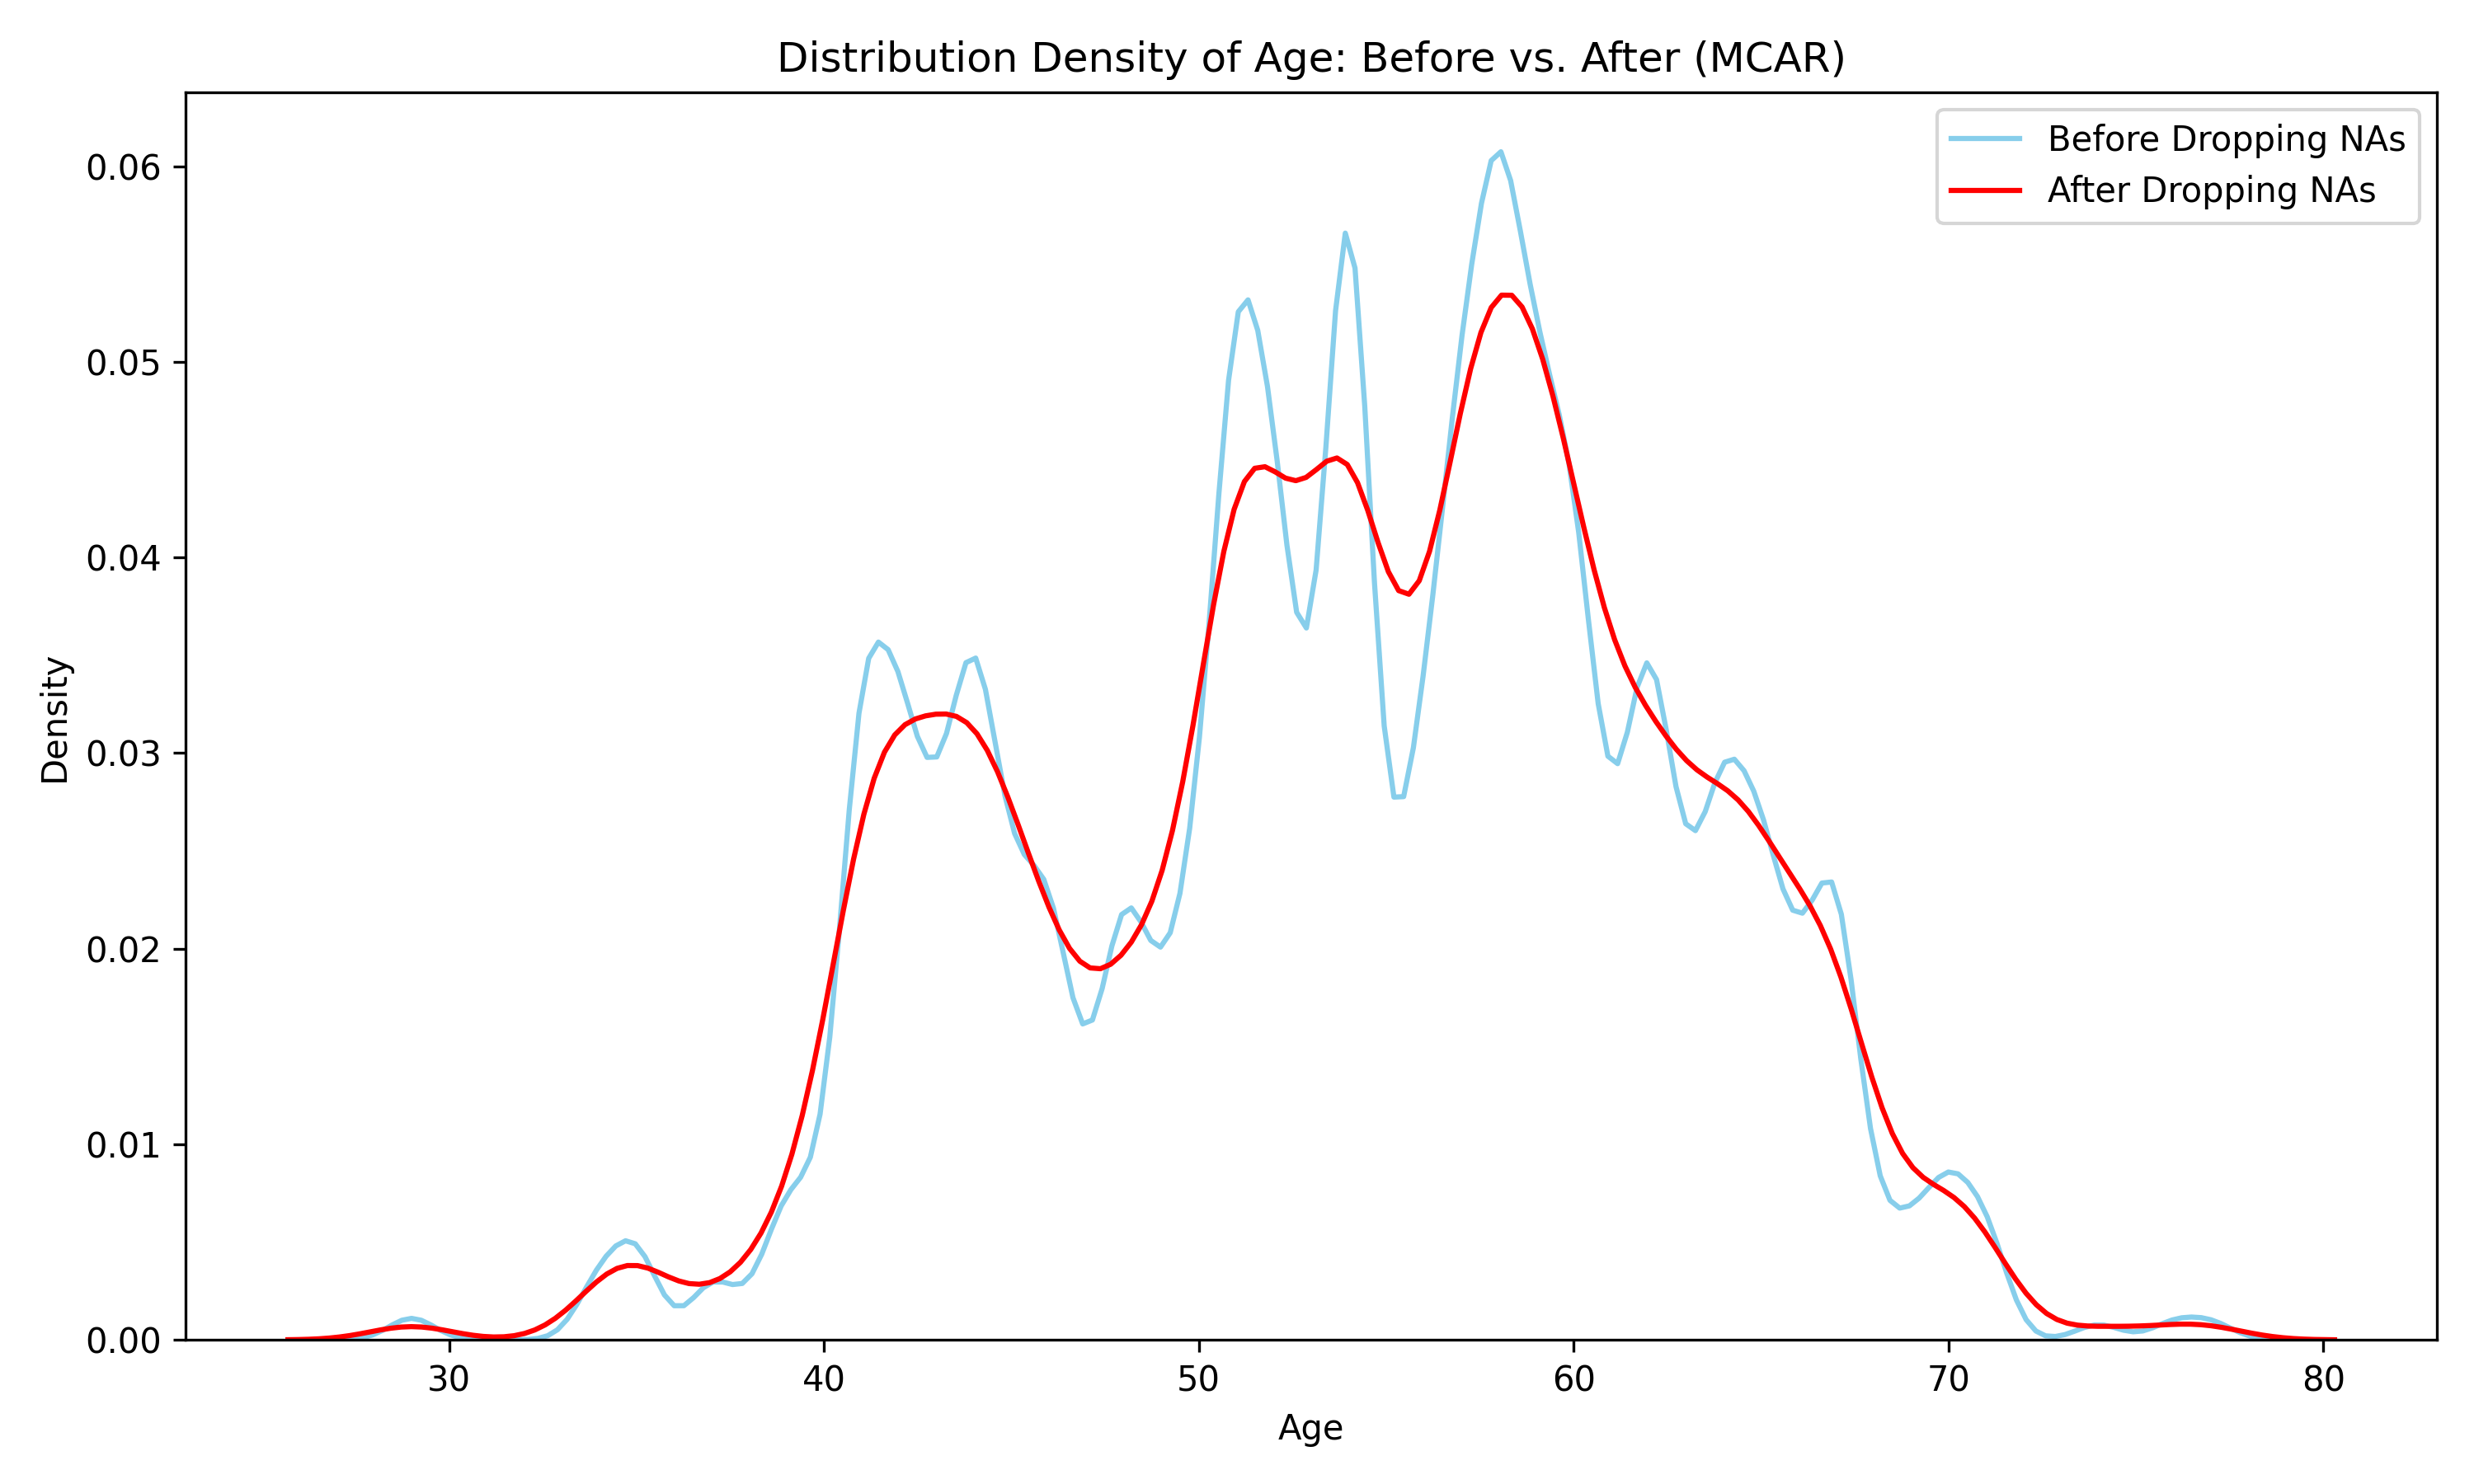
\includegraphics[width=0.8\textwidth]{distribution_lines_age_MCAR.png}
        \caption{MCAR mechanism Age distribution before and after dropping missing values}
    \label{fig:distribution_lines_age_MCAR}
\end{figure}

\paragraph{\textbf{Missing at Random (MAR)}}~\\ 
MAR is a missingness mechanism where missing values are related to other
observed values. Handling MAR is more nuanced as compared to MCAR as we can
introduce biases if we naively drop records containing missing values
\cref{fig:distribution_lines_age_MAR}.

Similar to MCAR, we most likely still do not need to know the underlying cause
of the missing values in order to impute the data as we can use Multivariate
imputation algorithms such as KNN and MICE \cite{buuren_mice_2011} to estimate these.

\begin{figure}[H]
    \centering
        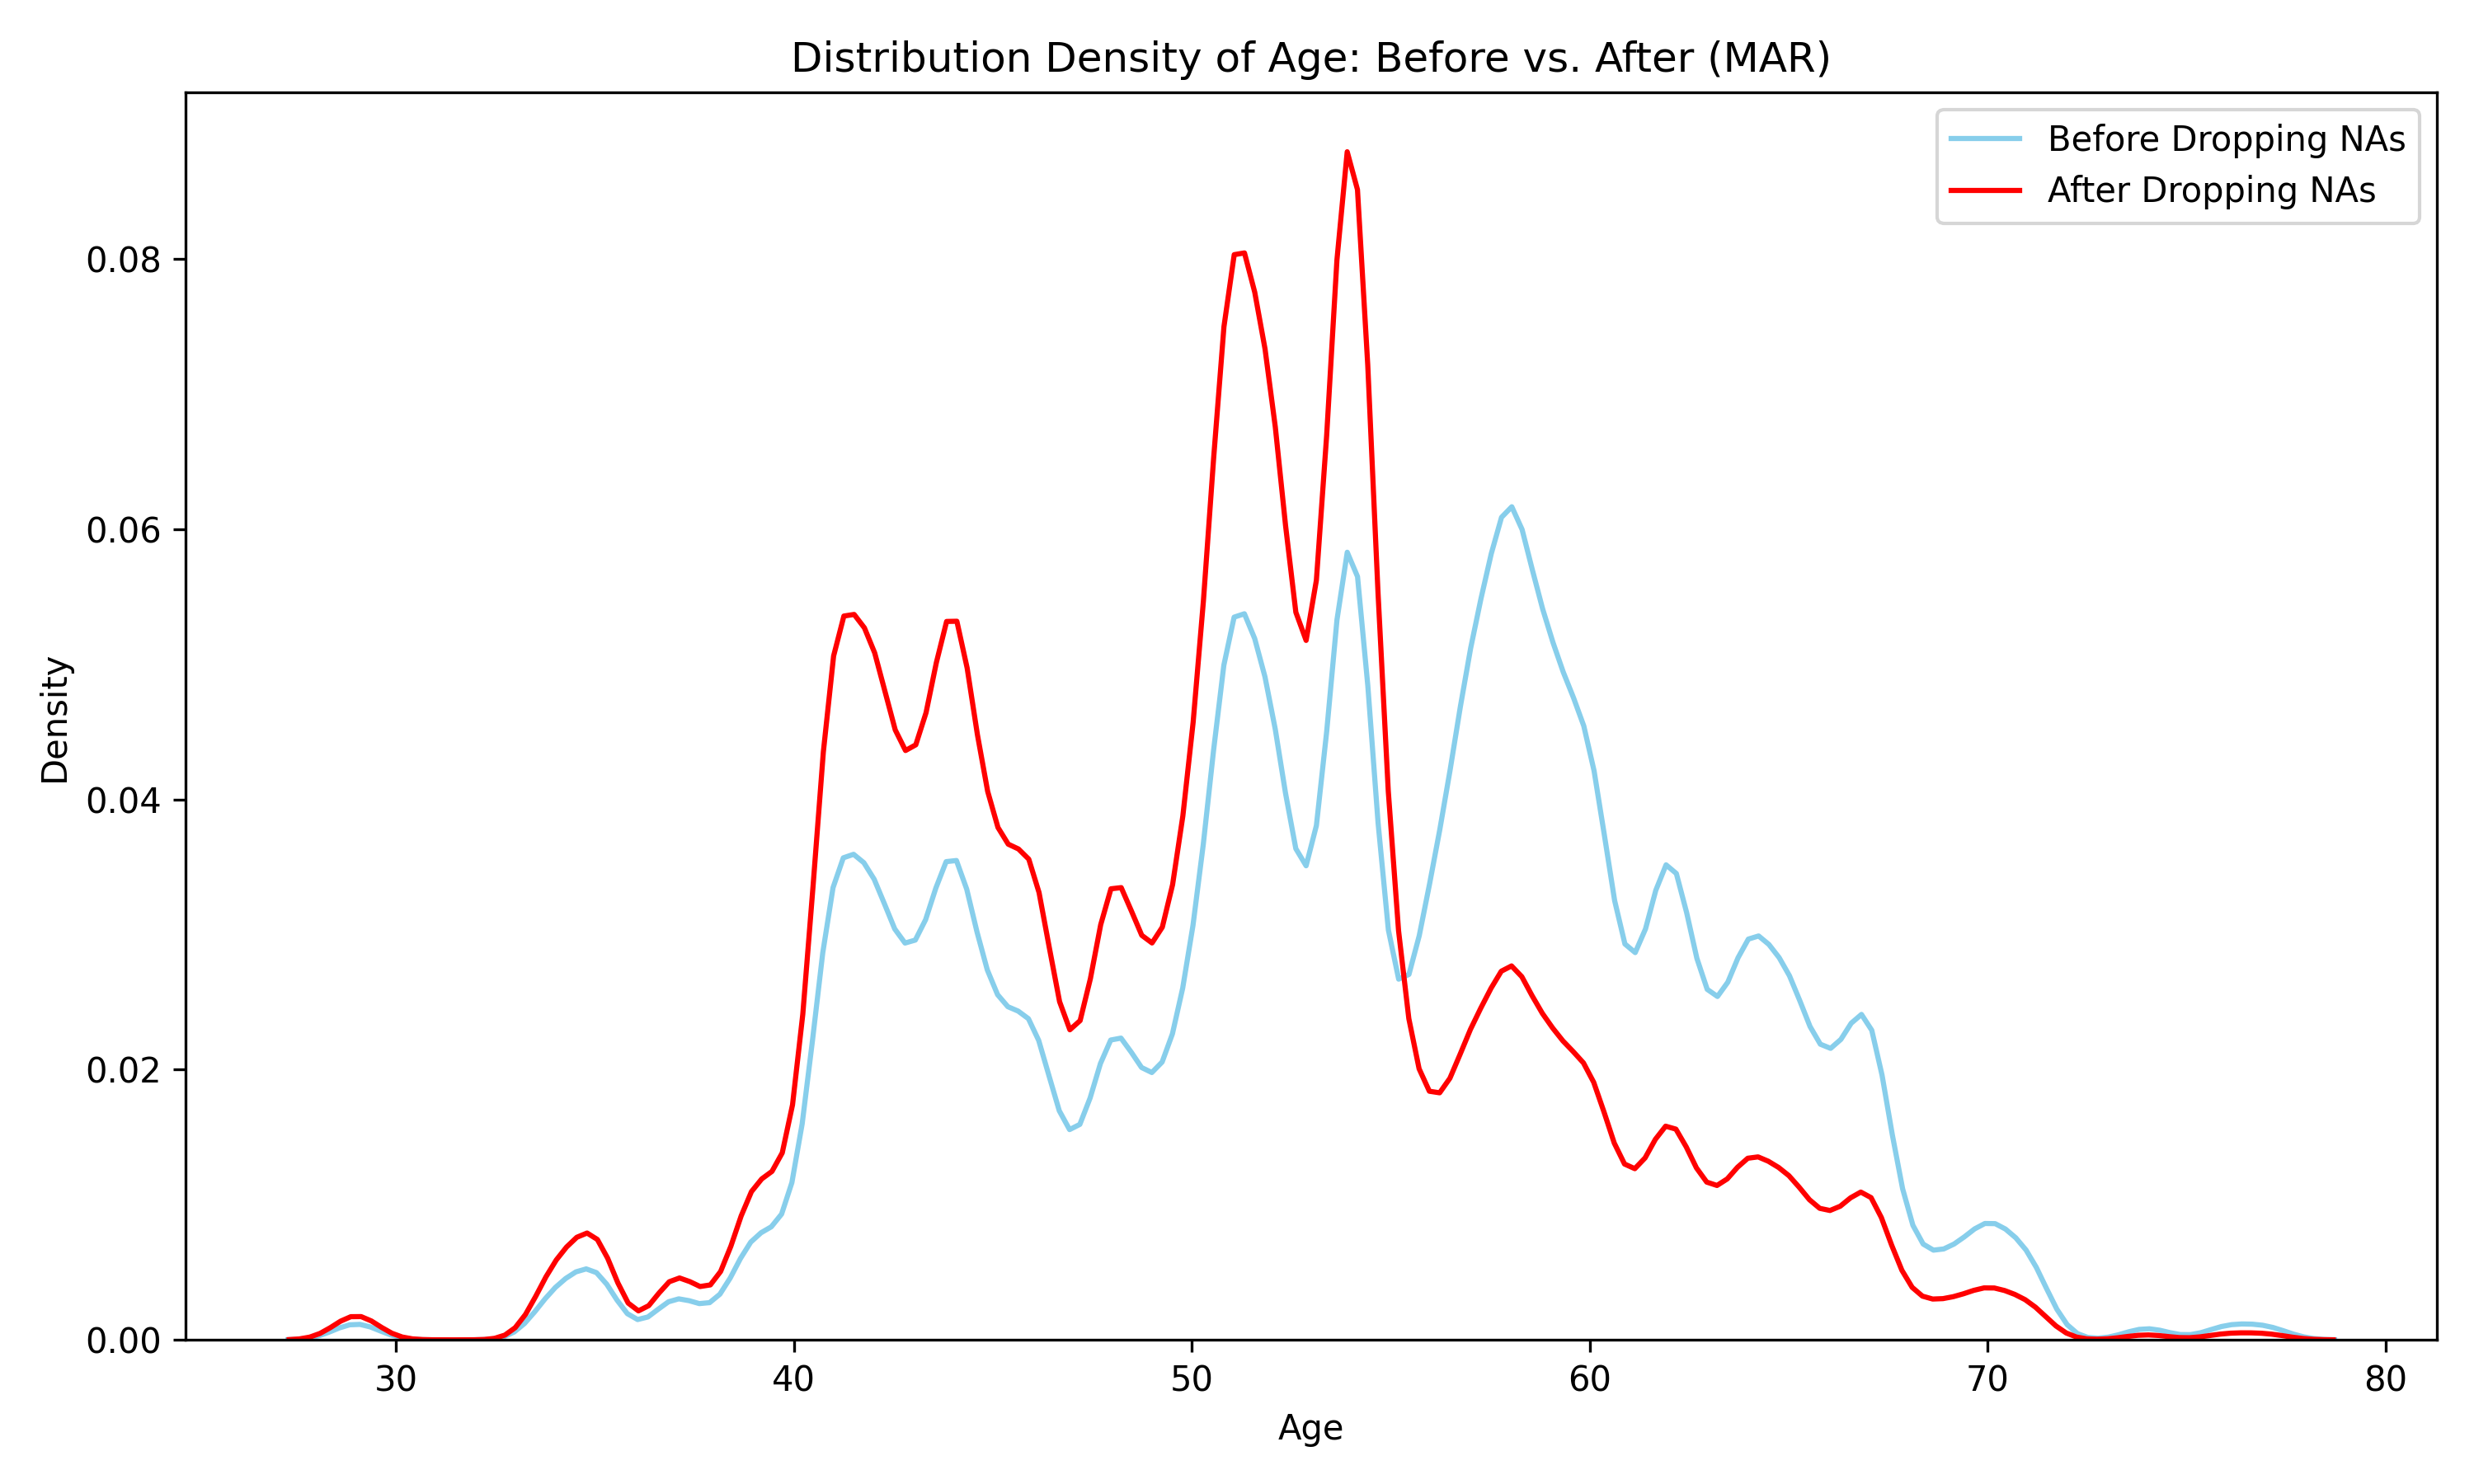
\includegraphics[width=0.8\textwidth]{distribution_lines_age_MAR.png}
        \caption{MAR mechanism Age distribution before and after dropping missing values}
    \label{fig:distribution_lines_age_MAR}
\end{figure}

\paragraph{\textbf{Missing Not at Random (MNAR)}}~\\ 
MNAR is a missingness mechanism where the likelihood of a value being missing
is dependent on unobserved values. Out of the three missingness mechanisms,
this is the most severe as knowledge of the underlying cause of the missing
data is required to perform data imputation. MNAR suggests there could be fault
in the data gathering process. WHO TO CITE FOR THIS?.

\subsubsection{Missingness patterns}
Missingness patterns are a derivation of \emph{missingness mechanism} that is
more easily identifiable and actionable by a data scientist working on a data
analytics task with missing variables. Fernstad \cite{fernstad_identify_2019}
defines three specific characteristics of missing data to look for.
\begin{enumerate}
        \item \textit{Amount Missing}
        \item \textit{Joint Missingness}
        \item \textit{Conditional Missingness}
\end{enumerate}

\paragraph{\textbf{Amount Missing}}~\\
The \textit{Amount missing} describes the percentage missing of a selected variable out of
all records in a dataset. This is useful to know in a practical sense as that
data engineers need to know what variables are worth imputing and discarding.
We can also use this to identify or dismiss the \textit{MCAR} missingness
mechanism for a variable. 

\begin{figure}[H]
    \centering
    \begin{subfigure}[H]{\textwidth}
        \centering
        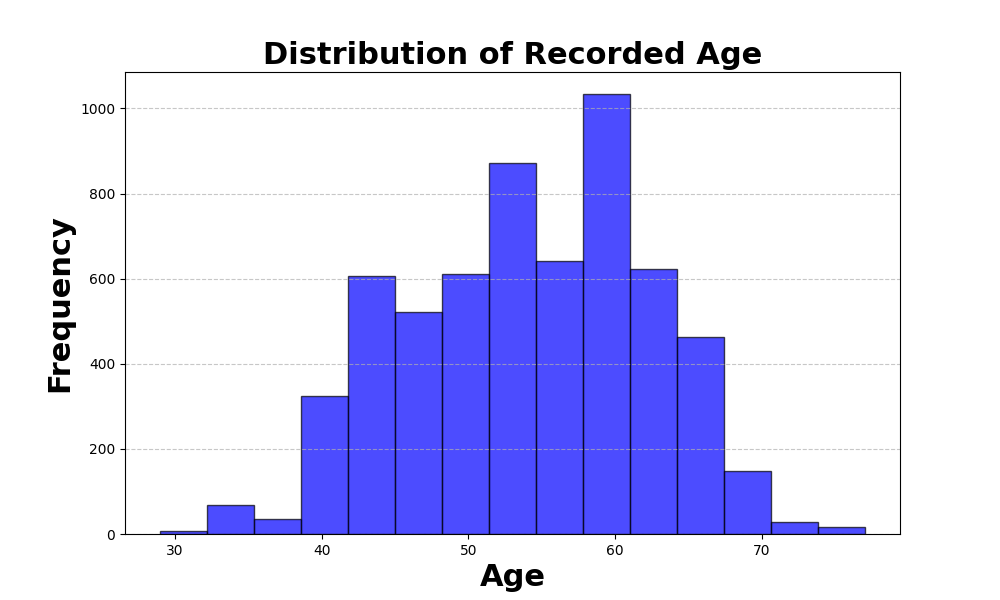
\includegraphics[width=\textwidth]{MCAR_recorded_age_distribution.png}
        \caption{Recorded age values.}
    \end{subfigure}\hfill
    \begin{subfigure}[H]{\textwidth}
        \centering
        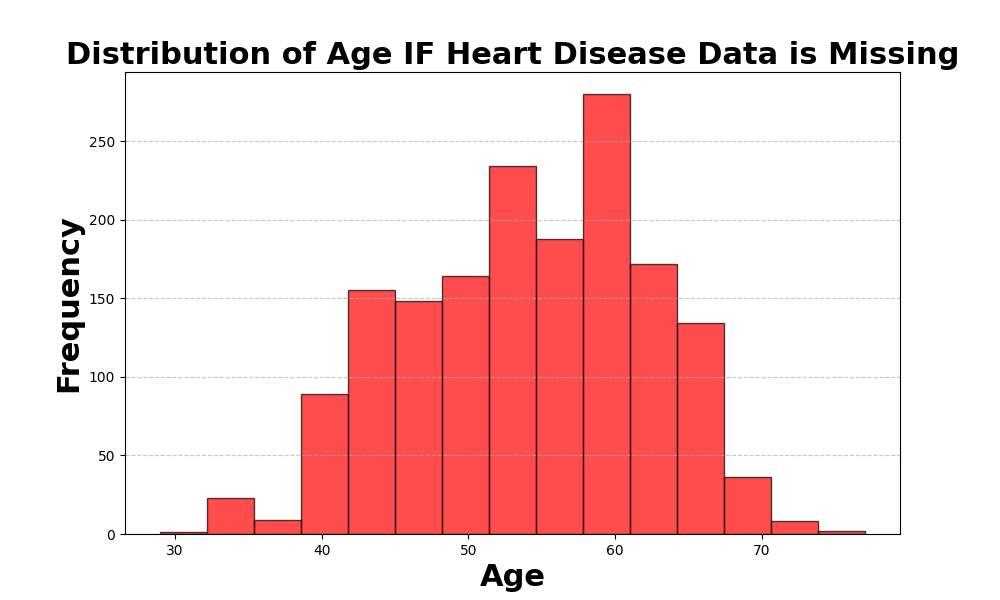
\includegraphics[width=\textwidth]{MCAR_missing_hd_age_distribution.png}
        \caption{Age when Heart Disease is missing.}
    \end{subfigure}
    \caption{Comparison of age distributions across the dataset; MCAR mechanism}
    \label{fig:MCAR_age_comparison}
\end{figure}

As seen in \cref{fig:MCAR_age_comparison}, the distribution of \textbf{Age} and
the distribution of \textbf{Age if Heart Disease is missing} show similar
distributions as mathematically described by a low Wasserstein distance of
\textbf{0.1174}. This indicates a high likelihood of the missingness mechanism
present being MCAR. 



\begin{figure}[H]
    \centering
    \begin{subfigure}[H]{\textwidth}
        \centering
        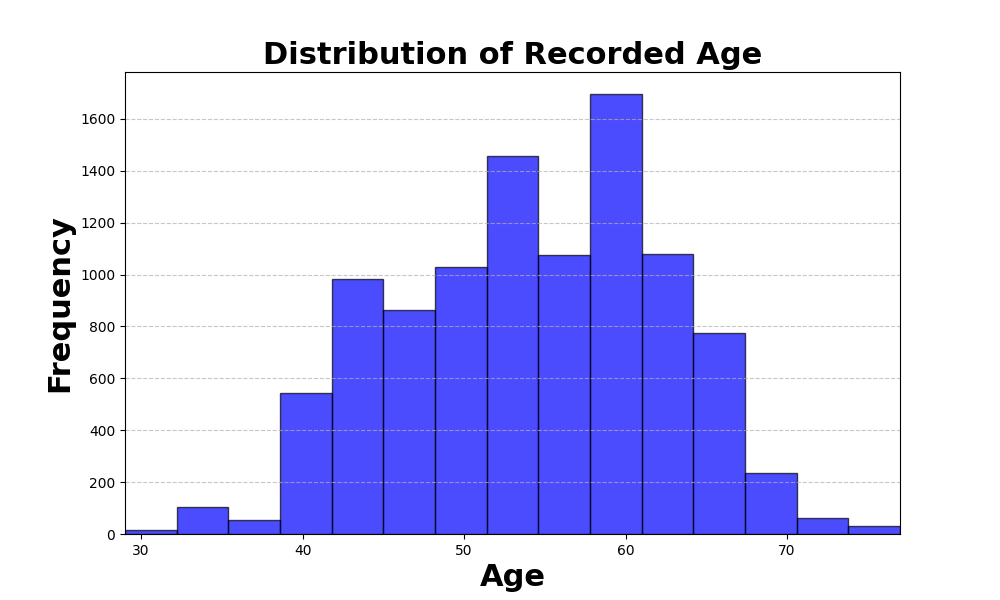
\includegraphics[width=\textwidth]{MAR_recorded_age_distribution.png}
        \caption{Recorded age values.}

    \end{subfigure}
    \begin{subfigure}[H]{\textwidth}
        \centering
        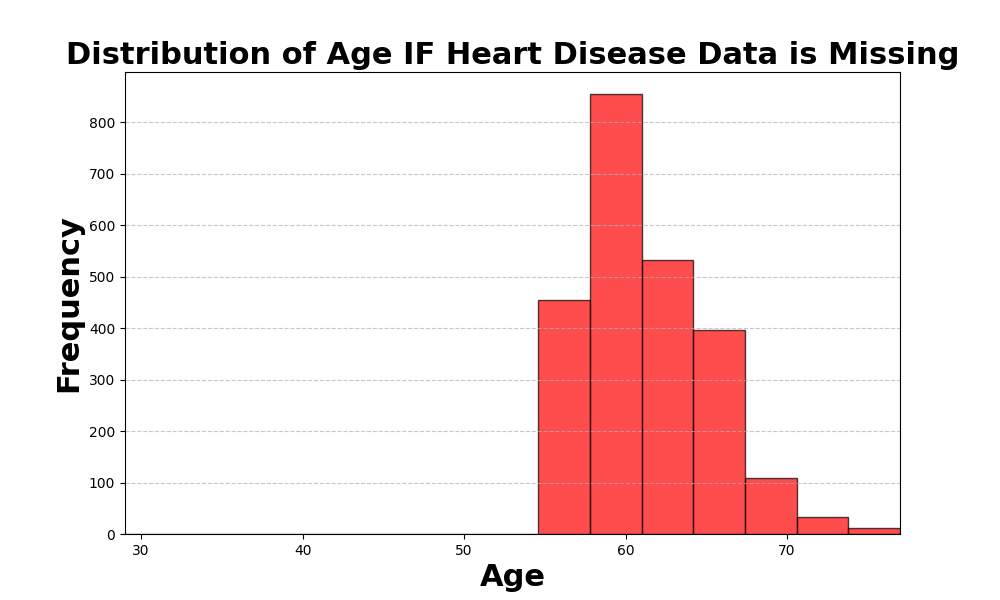
\includegraphics[width=\textwidth]{MAR_missing_hd_age_distribution.png}
        \caption{Age when Heart Disease is missing.}
    \end{subfigure}
    \caption{Comparison of age distributions across the dataset; MAR mechanism}
    \label{fig:MAR_age_comparison}
\end{figure}

Contrarily in \cref{fig:MAR_age_comparison} we get a Wasserstein distance of
\textbf{6.9925}, describing a large difference in distribution between the two
Age frequency histograms. For a data scientist practitioner, this can rule out
MCAR and they can look into verifying the nature of the missingness mechanism
of the missing variable. 



\paragraph{\textbf{Joint Missingness}} ~\\ 
A \textit{Joint missingness} pattern refers to the likelihood of a variable
being missing if one or more other variables are also missing. Finding evidence
of joint missingness, suggests the presence of the MNAR mechanism. This can be
expressed with the use of a heatmap. 

\begin{figure}[H]
    \centering
        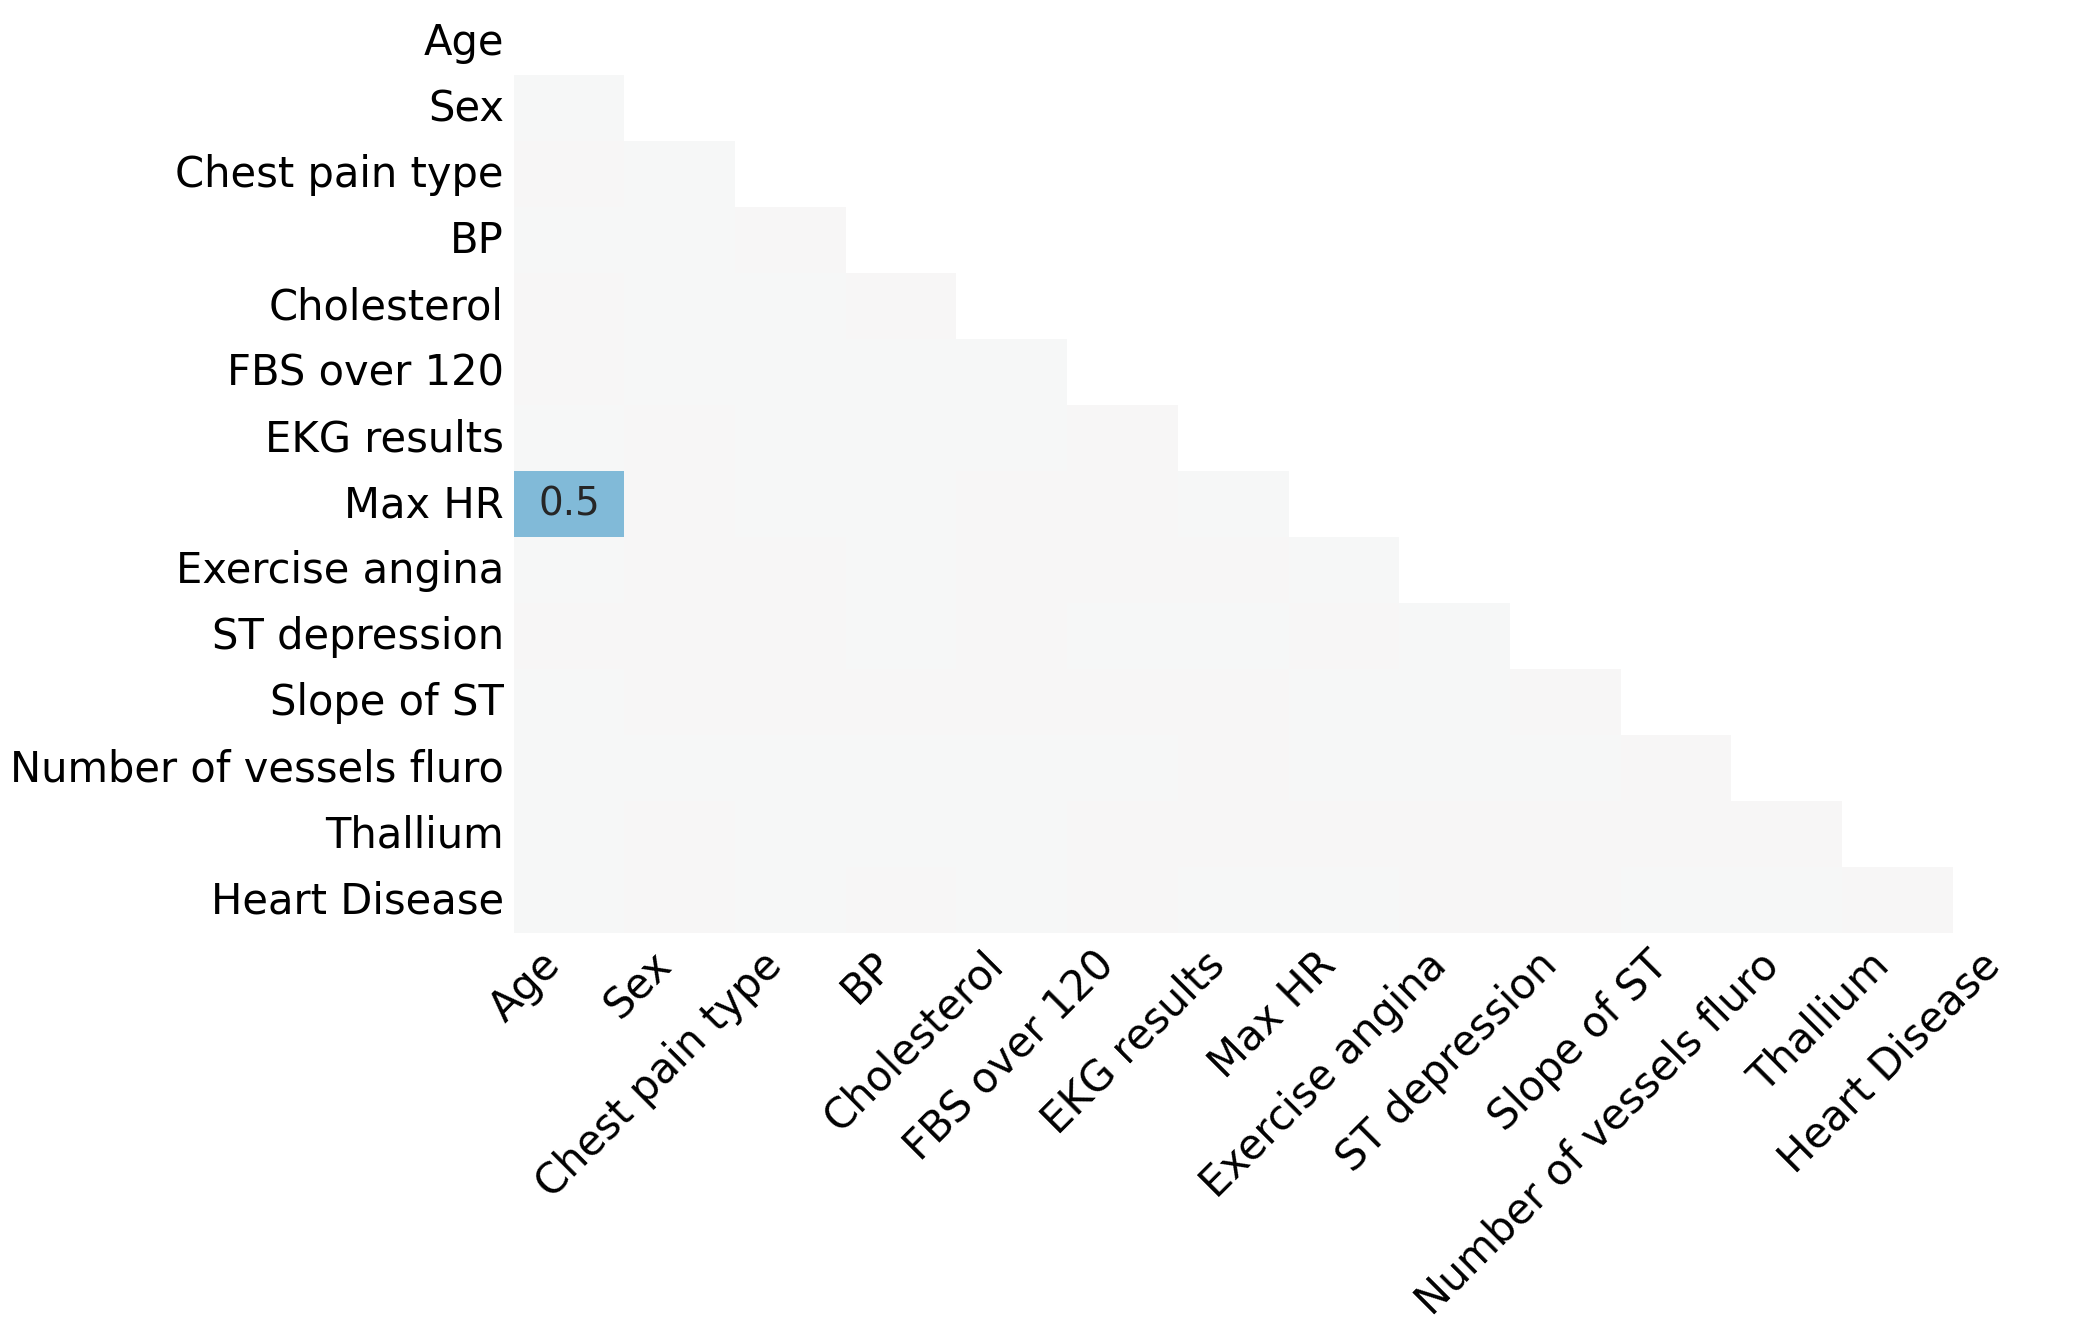
\includegraphics[width=0.9\textwidth]{JM.png}
        \caption{Joint Missingness depicted via Heatmap
        \cite{bilogur_residentmariomissingno_2026}}
    \label{fig:JM}
\end{figure}

For the given example \cref{fig:JM}, \textbf{30\%} of Age values are missing;
If Age is missing, \textbf{80\%} of Max Hr values are missing. MCAR was added
after at a rate of \textbf{20\%}. The blue intersecting block shows a nullity
correlation between Age and Max Hr of \textbf{0.5}.

\paragraph{\textbf{Conditional Missingness}} ~\\ 
A \textit{Conditional missingness} pattern refers to the likelihood of a
variable being missing depending on the value of another variable. This is more
tricky to visualize as instead of its likelihood of being missing being
dependent on the likelihood of other variables being missing as in
\textit{Joint Missingness}, we need a way to visualize the values of a variable
compared to the relative missingness of a variable. Finding evidence of
\textit{Conditional Missingness} suggests the presence of a MAR mechanism.

\begin{figure}[H]
    \centering
        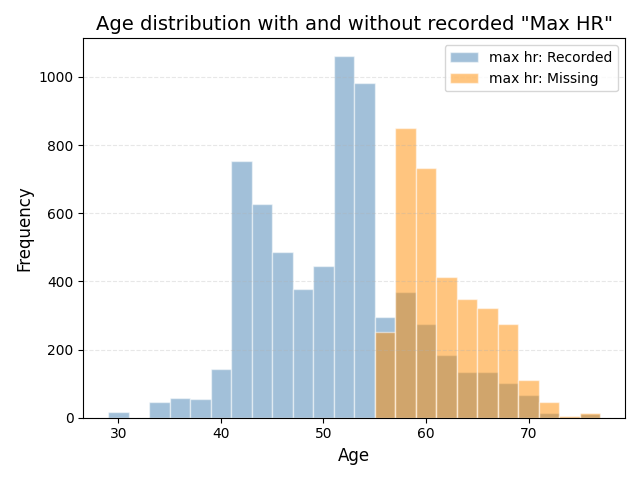
\includegraphics[width=0.9\textwidth]{conditional_missingness_MAR.png}
        \caption{Conditional missingness of Age dependent on Max HR}
    \label{fig:conditional_missingness_MAR}
\end{figure}

The above \cref{fig:conditional_missingness_MAR} is a synthetically created
example of conditional missingness with the following rules \ref{conditionalmissingness}: 

Let $M_i$ be the missingness indicator for the $i$-th observation, where $M_i =
1$ if $\text{Max\_HR}$ is missing and $M_i = 0$ if it is observed. Let $A_i$
represent the age of the individual. The missing data mechanism is defined as:

\begin{equation}
\label{conditionalmissingness}
P(M_i = 1 \mid A_i) = 
\begin{cases} 
    0.7 & \text{if } A_i > 55 \\
    0   & \text{if } A_i \le 55 
\end{cases}
\end{equation}

\subsection{Visualizing Missing Data}
Fernstad's study \cite{fernstad_identify_2019} into the effectiveness of
certain visualization methods in relation to how well participants are able to
identify missingness patterns can help make suggestions into what visualization
methods would be beneficial to provide in the implementation of \mica.
The user-study test how well participants are able to identify missingness
patterns with the use of three visualization methods. 

\begin{enumerate}
        \item Marginplot Matrix
        \item Parallel Coordinates
        \item Matrix Plot 
\end{enumerate}

Both Matrix plot and Parallel Coordinates performed significantly better as
compared to Marginplot in identifying missingness patterns \cite[Table
4]{fernstad_identify_2019}. Fernstad argues for the importance of clear
frequency representation as well as the benefits of not separating recorded and
unrecorded values in regard to being able to identify \textit{Conditional
Missingness}. 

\paragraph{\textbf{MissiG}} ~\\ 
With advancements made in Fernstad's previous study into visualization methods
for missing data \cite{fernstad_identify_2019}, Fernstad \textit{et al}. develops the novel
visualization MissiG \cite{fernstad_explore_2022} with an aim to make it easier
for data science practitioners identify missingness patterns in a dataset.

\begin{figure}[H]
    \centering
    \begin{subfigure}{0.45\textwidth}
        \centering
        
\includegraphics[width=\textwidth]{age.pdf}
        \caption{Age}
    \end{subfigure}
    \hfill
    \begin{subfigure}{0.45\textwidth}
        \centering
        
\includegraphics[width=\textwidth]{cholesterol.pdf}
        \caption{Cholesterol}
    \end{subfigure}
    \hfill
    \begin{subfigure}{0.45\textwidth}
        \centering
        \fbox{
\includegraphics[width=\textwidth]{stdepression.pdf}}
        \caption{ST depression}
    \end{subfigure}
    \hfill
    \begin{subfigure}{0.45\textwidth}
        \centering
        
\includegraphics[width=\textwidth]{maxhr.pdf}
        \caption{Max HR}
    \end{subfigure}
    \caption{MissiG implementation}
    \label{fig:MissiG}
\end{figure}

\cref{fig:MissiG} is an example implementation of MissiG. 

The glyphs are read as such: 
\begin{itemize}
        \item Red outline signified the selected variable.
        \item Blue histogram (left) shows the frequency of the variable.
        \item Blue bar (bottom right) shows the relative missingness of the variable.
        \item Red histogram (right) shows the frequency for the variable where the selected variable is missing.
        \item Red bar (bottom right) shows the joint missingness between the variable and the selected variable.
\end{itemize}


Following a user-study comparing how well users are able to identify
missingness patterns with MissiG, it is confirmed that MissiG was the users
preferred choice for identifying missingness patterns when compared to the use
of a Heatmap and Parallel Coordinates.

The uniquely interactive component of MissiG as well as its superior
performance for identifying missingness patterns makes this visualization
especially suited for use in \mica.



\subsection{Imputation Techniques}

\subsection{Previous Implementations}

\subsection{Technology Stack Evaluation}

\subsection{Requirements}

\subsubsection{Functional Requirements}
\subsubsection{Non-Functional Requirements}

\section{What Was Done and How}

\subsection{High-level Architecture Overview}
MICA is split into three software components \cref{fig:MICA architecture}. Each
component is dockerised for portability.
\begin{itemize}
        \item MICA API 
        \item Impute Handler
        \item Frontend Client
\end{itemize}

\begin{figure}[H]
    \centering
        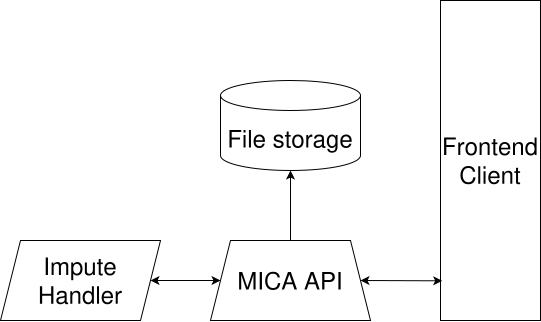
\includegraphics[width=0.8\textwidth]{MICA_architecture.pdf}
        \caption{MICA architecture}
    \label{fig:MICA architecture}
\end{figure}

\subsubsection{MICA API}
\mica provides a simple-to-use API for uploading, imputing and managing
versions of imputed datasets. This is routed through an NGINX reverse proxy to
provide in the future RESTful API version sub-routing. The MICA API handles the
imputation versioning system. This acts as the bridge between the frontend
client and the impute handler. \mica API design has allowed for the
addition of other currently unimplemented imputation methods without needing 
breaking changes.

\subsubsection{Impute Handler}
Imputation logic as well as data required to draw graphs in the frontend
client are calculated within the impute handler. Scikit-learn
\cite{pedregosa_scikit-learn_2011} handles KNN and MICE imputation. The
Scikit-learn imputation library was picked for use in \mica as the core
functions are written in PYX syntax and proven to be highly optimized. Custom
functions as well as custom JSON representations are used to send information
back to the MICA API; This includes a novel JSON standard for the MissiG
visualization. 

\subsubsection{Frontend Client}
This utilizes D3.js \cite{noauthor_d3d3_2026} for drawing and rendering SVG
chart components. D3.js was chosen as it provides low-level tooling to enable
the development of novel visualizations such as MissiG. To maintain a stateful
manner in the frontend, \mica uses React  \cite{noauthor_react_nodate}
+ MobX  \cite{noauthor_about_nodate} to cache results requested from the MICA
API. For low latency interactability, \mica uses Shadcn-ui
\cite{noauthor_shadcn-uiui_2026} for styling as it is performant.

\subsection{Imputation Versioning System}
MICA introduces a novel way to track dataset versions in regard to imputations
performed on said dataset.
\subsubsection*{The Problem}
The typical workflow of a data imputation task is an iterative process where
developers will need to create different versions of a dataset with varying
methods of imputation. With these different versions, in order to select the
best method of imputation, the user will need to create custom scripts
every time they would like to compare outputs. This process is tedious and
time-consuming. The process gets particularly complex when you have to keep
track of more than one imputation's difference between versions. 

For example, the below node diagram \cref{fig:nodegraph} depicts the history of imputations
performed on the dataset (root node). The cognitive overhead of keeping track
of the difference between nodes D and C's history can be prone to error due to
its complexity.

\begin{figure}[H]
    \centering
        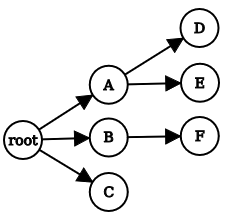
\includegraphics[width=0.5\textwidth]{nodegraph.png}
        \caption{Example version history node graph representation}
    \label{fig:nodegraph}
\end{figure}

\subsubsection*{The Solution}

When a request to impute a dataset is sent from the client to the MICA API, the
operations are done in the following order.
\begin{enumerate}
\item Request is sent to MICA API.
\item Request is validated and passed onto the impute handler.
\item Impute handler creates version of dataset and returns err code.
\item MICA API creates hash for new dataset version and stores information on imputation.
\item MICA API returns err code and new version history information to client.
\end{enumerate}

To store the history of a data imputation, \mica uses a hierarchical
strict tree structure. Since in some cases, imputation order matters, a tree
data structure is suited for this problem as it inherently stores child\\parent
information and no sideways or backwards connections are allowed.


\subsection{UI Implementation}
\mica's UI is split into three tabs that aims to push the user into a simple
linear workflow.
\begin{enumerate}
        \item Pre-imputation Analytics (MissiG view)
        \item Imputation tab
        \item Post-imputation Analytics (comparative visualizations) 
\end{enumerate}

All actions in \mica are accessible by a touchscreen interface. File names are
automatically generated based on imputations requested by the user as well as
manually editable if the user would wish to give a custom name for a particular
version of a dataset.

\subsubsection{Pre-Imputation Analytics}
\mica provides a custom react component implementation of both a singular
MissiG glyph and an abstraction for developers to be able to handle a group of
MissiG glyphs. Each MissiG glyph is clickable offering an interactive
visualization to the user. Both were developed in a stateless manner to allow
for greater modularity. See below \ref{MissiG_React_Component_Props}

\begin{program}[H]
\begin{verbatim}
interface MissigGlyphCardProps {
  columnSummary: ColumnSummary;
  setSelectedGlyphIdxOnClick: (idx: number) => void;
  selectedGlyphIdx?: number;
}

interface MissigGlyphProps {
  columnSummary: ColumnSummary;
  selectedGlyphIdx?: number;
}
\end{verbatim}
\caption{MissiG React Component Props}
\label{MissiG_React_Component_Props}
\end{program}

MICA API includes a custom data structure for describing a MissiG
visualization. Numeric and Categorical data is handled with different histogram
data structure implementations.

Due to \mica's requirement of being low latency, the design decision to cache
these results in the frontend client was taken for the cost of greater memory
usage. This is necessary as the MissiG visualization generates a joint
missingness histogram for every pair of variables. Consequently, the total
number of generated histograms scales quadratically, at \( O(n^2) \) , relative
to the number of variables. If we were to request the MICA API to load this
data for every access instance, the latency will become noticeable and cause
unneeded load on the MICA API and Impute Handler containers.

\subsubsection{Imputation}
\mica currently provides five imputations methods. Due to the modular design,
the addition of further imputation methods is trivial. 

For columnwise imputation, Mean, Median and Mode is provided. These were
implemented manually with the use of the python package Pandas
\cite{noauthor_pandas_nodate}.

\mica provides 2 multivariate imputation options; KNN and MICE. KNN has the
added parameter N nearest-neighbors for the user to adjust manually. MICE in
the future could be expanded to allow the user to select the estimator; In the
current implementation, this is defaulted to use the following 
\begin{verbatim}
    RandomForestRegressor(
        n_estimators=10,
        criterion="squared_error",
        max_depth=None,
        min_samples_split=2,
        min_samples_leaf=1,
        min_weight_fraction_leaf=0.0,
        max_features=1.0,
        max_leaf_nodes=None,
        min_impurity_decrease=0.0,
    )
\end{verbatim}

A feature-level missingness visualization was integrated into the column
selector table, an approach adapted from the "Profiler" imputer application
\cite{kandel_profiler_2012}. Other useful information such as feature name,
data type, Null count and Non-null count is displayed to the user. The
"Non-null count" badge indicator uses an orange-to-gray color transition to
denote the shift from sparse to complete data.

\begin{figure}[H]
    \centering
        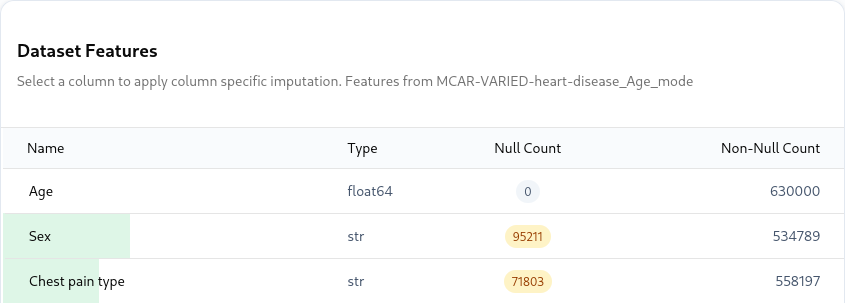
\includegraphics[width=\textwidth]{imputationtab_featuretable.png}
        \caption{\mica Imputation tab amount missing visualization}
\end{figure}

\subsubsection{Post-Imputation Analytics}
The imputation version history is represented in a timeline format going from
oldest at the top and newest at the bottom \cref{fig:commithistory}. For each
applied imputation, a new node is appended to the head of the commit history.
For each node on the commit history, a revert button is assigned to it; This
calls the MICA API endpoint that reverts history to a specific file hash. Doing
so will delete all children of this file hash in order to save storage. Each node
also has a dropdown to display cards showing applied imputations to that
particular version of the dataset, from oldest to newest imputation. A
comparison selector toggle is also provided, so the user can pick a dataset to
include in a comparison visualization. 

\begin{figure}[H]
    \centering
        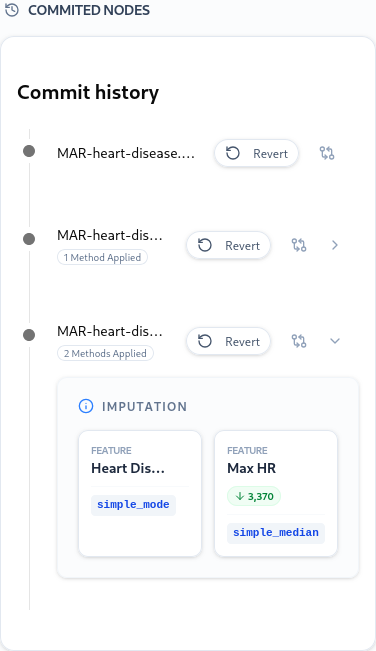
\includegraphics[width=0.5\textwidth]{commithistory.png}
        \caption{Commit history card}
        \label{fig:commithistory}
\end{figure}

As seen at the top of \cref{fig:filestab}, a drop-down card gives a list of important
information about the current head of the commit history.

\begin{itemize}
        \item File name 
        \item Dimensions
        \item Total null count
        \item Applied imputations
        \item Column names, types and null counts
\end{itemize}

As a way to interface with the currently uncommitted versions of the imputed
dataset, a record's table is displayed \cref{fig:imputation_records}. For each
created version, the user is given four options. apply imputation, download
version, discard version and toggle comparison selector. 
\begin{description}
    \item[Apply imputation] This action performs a commit action, clearing the
            staging area and appending the selected node to the head of the
            commit history. 

    \item[Download version] Creates a download link for version of imputed
            dataset.

    \item[Discard version] Permanently removes the uncommitted version from the
            interface and backend file storage.

    \item[Toggle comparison selector] Enables a side-by-side view to visualize
            differences between any two versions of the dataset.
\end{description}

Each record has a dropdown menu to display a history of imputations performed
on it including diff values, type of imputation performed and feature imputed
for each imputation card. 

\begin{figure}[H]
    \centering
        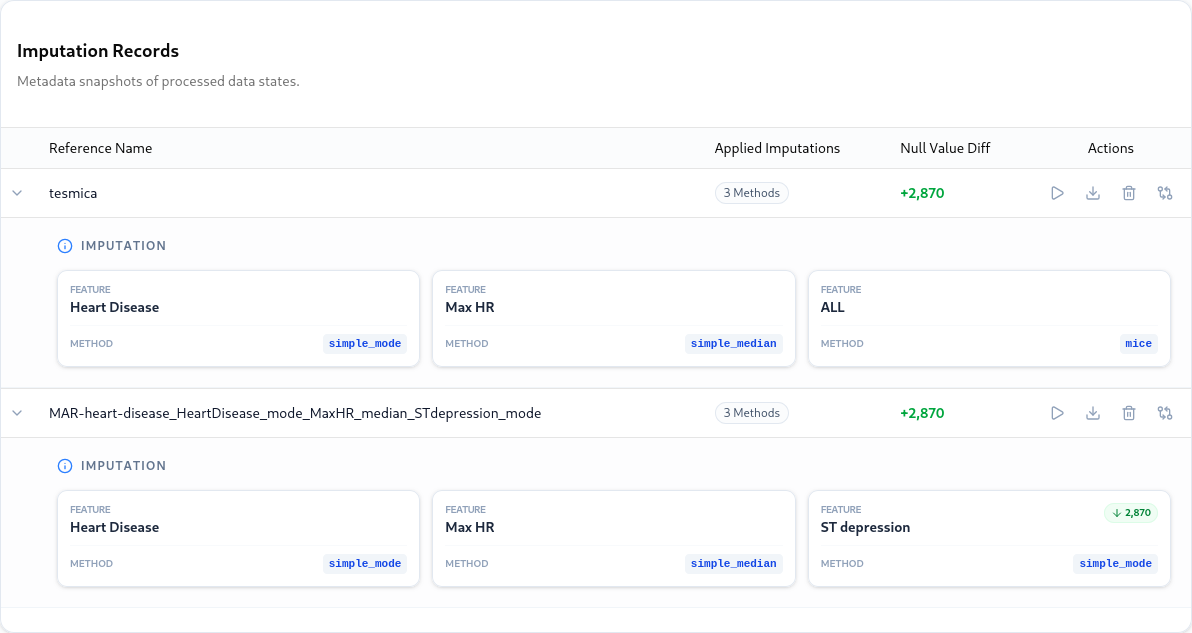
\includegraphics[width=\textwidth]{filetabrecords.png}
        \caption{Imputation record's table}
        \label{fig:imputation_records}
\end{figure}

The comparison selector toggle was designed to work in conjunction with both
the commit history and the imputation records table. This allows users to
compare newly created uncommitted records with previous versions of the
dataset.

When two dataset versions are selected by the user, the user is given the
option to open a dialog to compare the two selected datasets. This is indicated
to the user by an enabled or disabled button. 

The first visualization presented to the user is an interactive parallel
coordinates graph comparison widget \cref{fig:parallelCoordinatesCompare}. A
random sample of indexes is taken out of both datasets and displayed; matching
indexes are used as the difference in each graph should only be in features
which have changed. Each are overlaid in contrasting blue and red. Three
buttons are provided for the user to switch between displaying both graphs or
either of the graphs by itself. The interface assists in the detection of
meaningful correlations, providing the clarity necessary to differentiate
signal from data noise

The main drawback of using this visualization is that order matters; it can be
difficult for the user to spot correlations when the two features with
correlations are on opposite ends of the graph. This has been mitigated by the
implementation of the drag and drop reordering feature. With this feature,
users are able to try out different orders of features.

% TODO do missingnessas matrix, and stats section of comparison dialog
The second visualization presented to the user is a missingness matrix dialog
\cref{fig:missingnessmatrix}.

\subsubsection{Example User-flow}

\subsection{Synthetic Data Generation}

\section{Results and Evaluation}
\subsection{System Outputs}      
\subsection{Limitations}
\subsection{Performance}

\section{Conclusion}
\subsection{Aims and Objectives}
\subsection{Future Work}

\newpage
\section{References}
\bibliographystyle{plainnat}
\bibliography{references}

\section{Appendix}
\appendix

\section{MICA API implementations}
\begin{program}[H]
\begin{verbatim}
type FileNode struct {
        UUID        uuid.UUID
        Path        string
        Imputations []Imputation
}

type Imputation struct {
        Feature string           
        Method  ImputationMethod 
}
\end{verbatim}
\caption{Internal MICA API implementation data structure for imputation versioning system}
\end{program}

\begin{program}[H]
\begin{verbatim}
type BasicInfo struct {
	UUID        uuid.UUID    `json:"uuid"`
	Filename    string       `json:"filename"`
	ColumnInfo  []ColumnInfo `json:"columns"`
	Shape       [2]int       `json:"shape"`
	Imputations []Imputation `json:"imputations"`
}

ParentHistory []model.BasicInfo `json:"parent_history"`
\end{verbatim}
\caption{Version history JSON structure}
\end{program}

\section{MICA UI}
\begin{figure}[H]
    \centering
        \wideimage{MissiGSC.png}
        \caption{MissiG visualization implementation}
\end{figure}

\begin{figure}[H]
    \centering
        \wideimage{imputationtab.png}
        \caption{\mica imputation tab}
\end{figure}

\begin{figure}[H]
    \centering
        \wideimage{filestab.png}
        \caption{\mica file management and comparison tab}
        \label{fig:filestab}
\end{figure}

\begin{figure}[H]
    \centering
        \wideimage{parallelCoordinatesCompare.png}
        \caption{Parallel Coordinates graph comparison component with drag and
        drop feature reordering}
        \label{fig:parallelCoordinatesCompare}
\end{figure}

\begin{figure}[H]
    \centering
        \wideimage{missingnessmatrix.png}
        \caption{Missingness Matrix comparison with on hover tooltip}
        \label{fig:missingnessmatrix}
\end{figure}

\end{document}

